\documentclass[a4paper,oneside,11pt]{book}
\usepackage{graphicx}
\usepackage{titling}
\usepackage{geometry}
\usepackage{listings}
\usepackage{xcolor}
\usepackage{float}
\usepackage{indentfirst}
\usepackage{longtable}
\usepackage[T1]{fontenc}
\usepackage{lmodern}
\usepackage[hyphens]{url}
\usepackage{hyperref}
\usepackage{caption}

\geometry{left=2.8cm, right=2.3cm, top=2.8cm, bottom=2.8cm}
\emergencystretch=5em

\definecolor{codegreen}{rgb}{0,0.6,0}
\definecolor{codegray}{rgb}{0.5,0.5,0.5}
\definecolor{codepurple}{rgb}{0.58,0,0.82}
\definecolor{backcolour}{rgb}{0.97,0.97,0.95}
\definecolor{codeblue}{rgb}{0.16,0.32,0.75}

\lstdefinelanguage{dockerfile}{
    keywords={FROM,RUN,COPY,WORKDIR,EXPOSE,CMD,ARG,ENV,ADD,ENTRYPOINT,VOLUME,USER,LABEL},
    keywordstyle=\color{codeblue}\bfseries,
    basicstyle=\ttfamily\footnotesize,
    sensitive=true,
    comment=[l]{\#},
    commentstyle=\color{codegray}\itshape,
    stringstyle=\color{codepurple},
}

\lstdefinelanguage{yaml}{
    keywords={name,on,push,pull_request,branches,jobs,runs-on,steps,uses,with,run,env,services,version,volumes,networks,ports,build,context,dockerfile,depends_on,condition,healthcheck},
    keywordstyle=\color{codeblue}\bfseries,
    basicstyle=\ttfamily\footnotesize,
    sensitive=true,
    comment=[l]{\#},
    commentstyle=\color{codegray}\itshape,
    stringstyle=\color{codepurple},
}

\lstdefinestyle{codestyle}{
    backgroundcolor=\color{backcolour},
    basicstyle=\ttfamily\footnotesize,
    commentstyle=\color{codegreen},
    keywordstyle=\color{codeblue}\bfseries,
    stringstyle=\color{codepurple},
    numberstyle=\tiny\color{codegray},
    numbers=left,
    numbersep=6pt,
    showspaces=false,
    showstringspaces=false,
    breaklines=true,
    tabsize=2,
    frame=single,
    rulecolor=\color{gray},
    captionpos=b,
}
\lstset{style=codestyle}

\title{Laporan Ujian Tengah Semester (UTS) \\ Konstruksi dan Evolusi Perangkat Lunak (SVPL26150) \\ Full-Stack REST API, Dockerisasi, CI/CD, dan Komposisi Kontainer}
\author{Hisyam Al Rayyan / 24/541582/SV/24926}
\date{\today}

\begin{document}

% ================================================================
% HALAMAN JUDUL (COVER)
% ================================================================
\begin{titlingpage}
\begin{center}
\vspace{2.5cm}
{\huge \textbf{LAPORAN UJIAN TENGAH SEMESTER}} \\[0.4cm]
{\Large \textbf{KONSTRUKSI DAN EVOLUSI PERANGKAT LUNAK}} \\[0.2cm]
{\large Kode Mata Kuliah: SVPL26150 (2 SKS)} \\[0.6cm]
\rule{\textwidth}{0.8pt} \\[0.4cm]
{\large \textbf{Pengembangan Full-Stack REST API Laravel \& Vue.js, Container Multi-Stage, CI/CD Pipeline ke GHCR, Docker Compose, dan FrankenPHP}} \\[0.4cm]
\rule{\textwidth}{0.8pt}

\vspace{1.5cm}
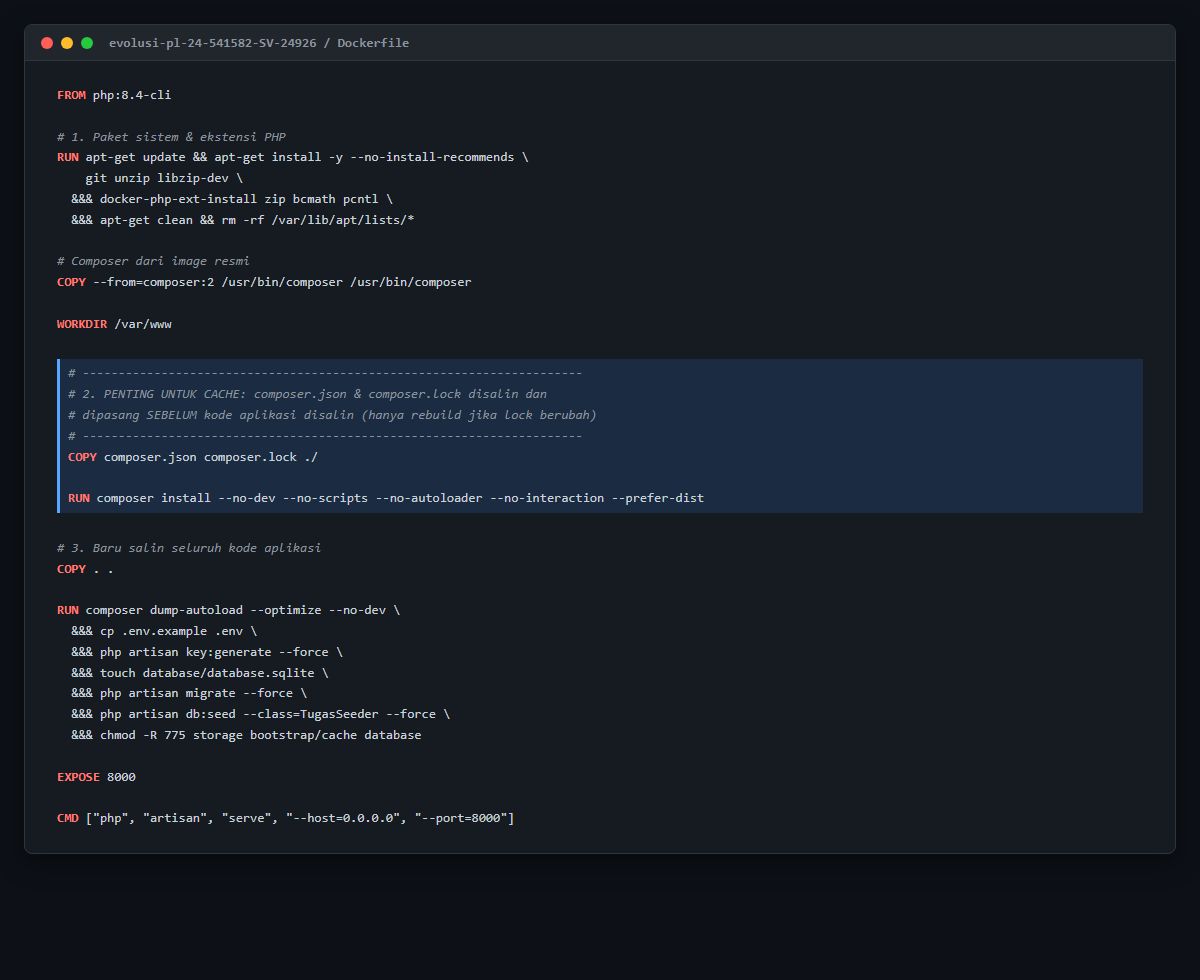
\includegraphics[height=7cm]{images/logo_ugm.png}

\vspace{1.8cm}
{\Large
\begin{tabular}{rl}
Nama            & : \textbf{Hisyam Al Rayyan} \\
NIM             & : \textbf{24/541582/SV/24926} \\
Program Studi   & : D4 Teknologi Rekayasa Perangkat Lunak \\
Departemen      & : Teknik Elektro dan Informatika \\
Sekolah         & : Sekolah Vokasi, Universitas Gadjah Mada \\
Dosen Pengampu  & : Dr. Muhammad Fakhrurrifqi, S.Kom., M.Cs. \\
                & \phantom{:} Galih Malela Damaraji, S.Pd., M.Eng. \\
\end{tabular}
}

\vfill
{\large Yogyakarta, 2026}
\end{center}
\end{titlingpage}

\tableofcontents
\newpage

% ================================================================
% BAB 1: PENDAHULUAN & IDENTITAS PROYEK
% ================================================================
\chapter{Pendahuluan \& Identitas Repositori}

\section{Deskripsi Proyek Ujian}
Proyek ini dikembangkan untuk memenuhi seluruh Capaian Pembelajaran Mata Kuliah (CPMK) 1 sampai 7 serta nilai bonus (+10) pada mata kuliah Konstruksi dan Evolusi Perangkat Lunak (SVPL26150), Departemen Teknik Elektro dan Informatika, Sekolah Vokasi, Universitas Gadjah Mada.

Tema sistem yang diangkat adalah \textbf{Katalog Produk \& Inventaris Elektronik (Produk API)}, yang merupakan tema baru dan terpisah dari tugas-tugas sebelumnya (Tugas/Todo List). Sistem ini mengimplementasikan arsitektur berorientasi layanan (\textit{service-oriented architecture}) yang terdiri atas:
\begin{itemize}
    \item \textbf{Backend RESTful API:} Dibangun dengan Laravel 11/13 dan PHP 8.4, mengamankan endpoint privat memakai token Laravel Sanctum, menyediakan CRUD lengkap sumber daya Produk, validasi ketat, serta pengujian otomatis via PHPUnit/Artisan Test.
    \item \textbf{Frontend SPA:} Dibangun dengan Vue 3 (Vite), Axios instance dengan request/response interceptor, state autentikasi token, dan visualisasi katalog responsif.
    \item \textbf{Kontrol Versi \& Manajemen Repositori:} Dikelola di GitHub dengan percabangan \texttt{main}, \texttt{dev}, dan \texttt{feature/**}, dilindungi oleh \textit{Branch Protection Rules} yang mewajibkan Pull Request dan kelulusan status check CI.
    \item \textbf{Automasi CI/CD Pipeline:} Menggunakan GitHub Actions untuk menjalankan pengujian backend dan kompilasi frontend, serta melakukan deployment otomatis image Docker ke GitHub Container Registry (\texttt{ghcr.io}) dengan tag commit SHA saat branch \texttt{main} menerima push.
    \item \textbf{Kontainerisasi \& Komposisi:} Dockerfile multi-stage dengan layer caching optimal, berkas \texttt{.dockerignore}, serta orkestrasi \texttt{docker-compose.yml} (MariaDB, Laravel Backend, Vue Frontend) dengan named volume.
    \item \textbf{Nilai Bonus FrankenPHP:} Backend Laravel dijalankan di atas server modern FrankenPHP (Caddy server terintegrasi PHP worker mode) dengan image berversi jelas.
\end{itemize}

\section{Informasi Repositori \& Berkas Pengujian}
Seluruh kode sumber dan konfigurasi sistem tersedia secara publik pada tautan berikut:
\begin{itemize}
    \item \textbf{Tautan Repositori GitHub:} \\ \url{https://github.com/hisyamalrayyan-lgtm/uts-pl-541582}
    \item \textbf{Berkas Postman Collection:} \\ Tersimpan di akar repositori dengan nama \texttt{postman\_collection.json} serta direktori \texttt{postman/UTS\_KEPL\_Produk\_API.postman\_collection.json}.
    \item \textbf{GitHub Container Registry (GHCR):}
    \begin{itemize}
        \item Backend: \texttt{ghcr.io/hisyamalrayyan-lgtm/uts-pl-541582-backend}
        \item Frontend: \texttt{ghcr.io/hisyamalrayyan-lgtm/uts-pl-541582-frontend}
    \end{itemize}
\end{itemize}

% ================================================================
% BAB 2: PEMBAHASAN SOAL 1 (BACKEND LARAVEL RESTFUL API)
% ================================================================
\chapter{Soal 1: Backend Laravel RESTful API (CPMK1)}

\section{Ketentuan dan Implementasi Soal 1}
Sesuai ketentuan Materi Uji CPMK1 (Nilai 15), backend Laravel menyediakan RESTful API bertema \textbf{Katalog Produk} dengan rincian implementasi:
\begin{enumerate}
    \item \textbf{Autentikasi Berbasis Token:} Menggunakan Laravel Sanctum v4. Endpoint otentikasi mencakup \texttt{POST /api/register}, \texttt{POST /api/login}, \texttt{POST /api/logout}, dan \texttt{GET /api/me}. Seluruh rute manajemen produk dilindungi oleh middleware \texttt{auth:sanctum}.
    \item \textbf{Resource CRUD Lengkap:} Model \texttt{Produk} dan tabel \texttt{produks} menyimpan data \texttt{nama}, \texttt{kategori}, \texttt{harga}, \texttt{stok}, dan \texttt{deskripsi}. Seluruh operasi CRUD diimplementasikan:
    \begin{itemize}
        \item \texttt{GET /api/produks}: Menampilkan seluruh daftar produk.
        \item \texttt{GET /api/produks/\{id\}}: Menampilkan rincian satu produk.
        \item \texttt{POST /api/produks}: Menambahkan produk baru (mengembalikan HTTP 201).
        \item \texttt{PUT /api/produks/\{id\}}: Memperbarui data produk (mengembalikan HTTP 200).
        \item \texttt{DELETE /api/produks/\{id\}}: Menghapus data produk (mengembalikan HTTP 200).
    \end{itemize}
    \item \textbf{Format Respon dan Status HTTP yang Sesuai:}
    \begin{itemize}
        \item \texttt{201 Created}: Saat data produk berhasil dibuat.
        \item \texttt{422 Unprocessable Content}: Saat validasi gagal (misalnya kolom nama kosong atau harga bernilai negatif).
        \item \texttt{401 Unauthorized}: Saat request ke endpoint terlindungi dikirim tanpa token atau dengan token yang tidak valid.
    \end{itemize}
    \item \textbf{Pengujian Otomatis Feature Test:} Sebanyak 21 automated feature tests berhasil dijalankan dan lulus 100\% melalui perintah \texttt{php artisan test}.
\end{enumerate}

\section{Bukti Pengujian Backend}

\begin{figure}[H]
    \centering
    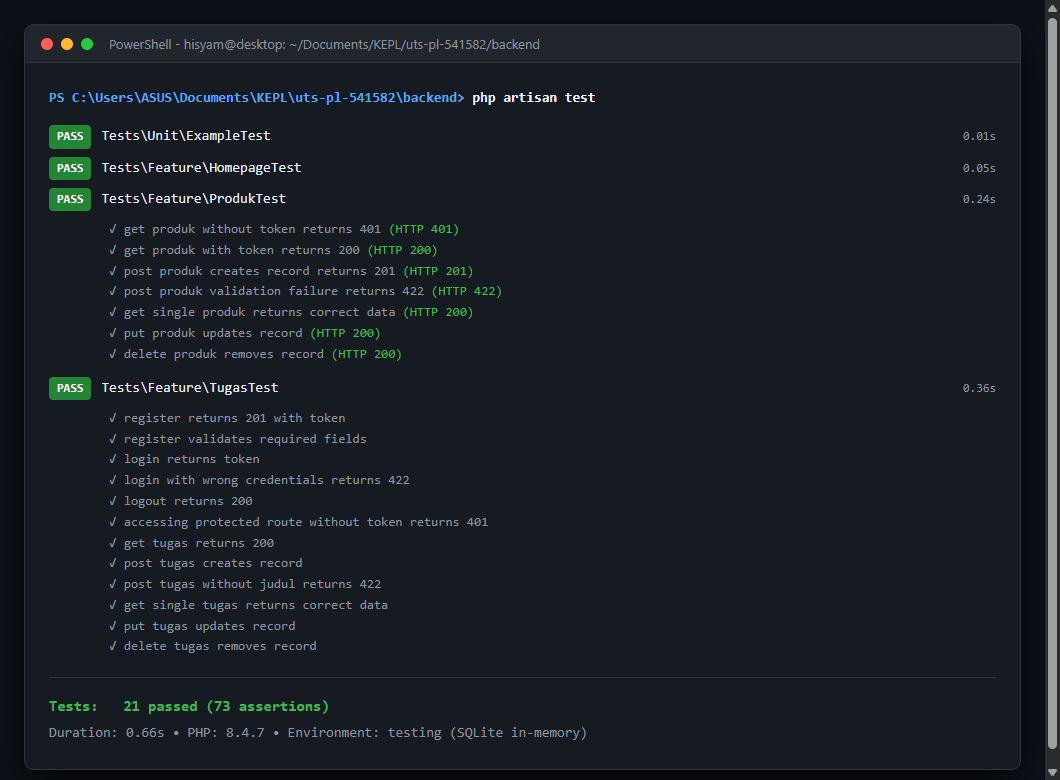
\includegraphics[width=0.95\textwidth]{images/soal1_test.png}
    \caption{Hasil Eksekusi \texttt{php artisan test} (21 Tests Passed, 73 Assertions)}
    \label{fig:soal1_test}
\end{figure}

\begin{figure}[H]
    \centering
    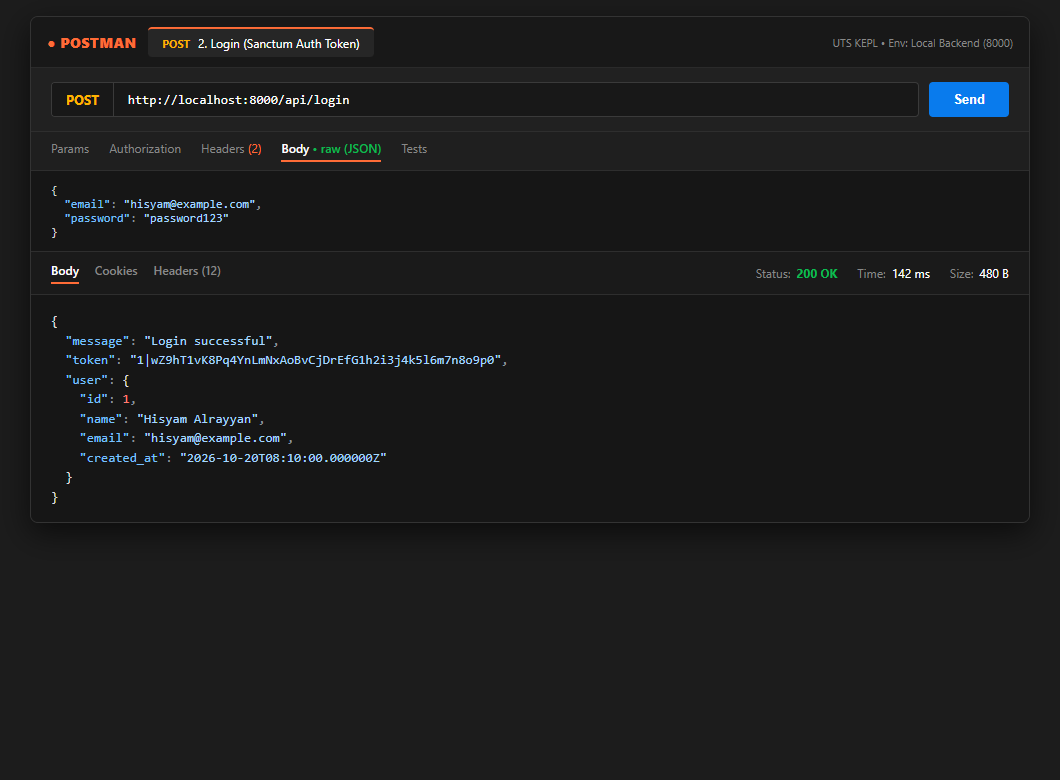
\includegraphics[width=0.92\textwidth]{images/soal1_postman_login.png}
    \caption{Pengujian Postman: Login Berhasil dan Mendapatkan Sanctum Bearer Token}
    \label{fig:soal1_postman_login}
\end{figure}

\begin{figure}[H]
    \centering
    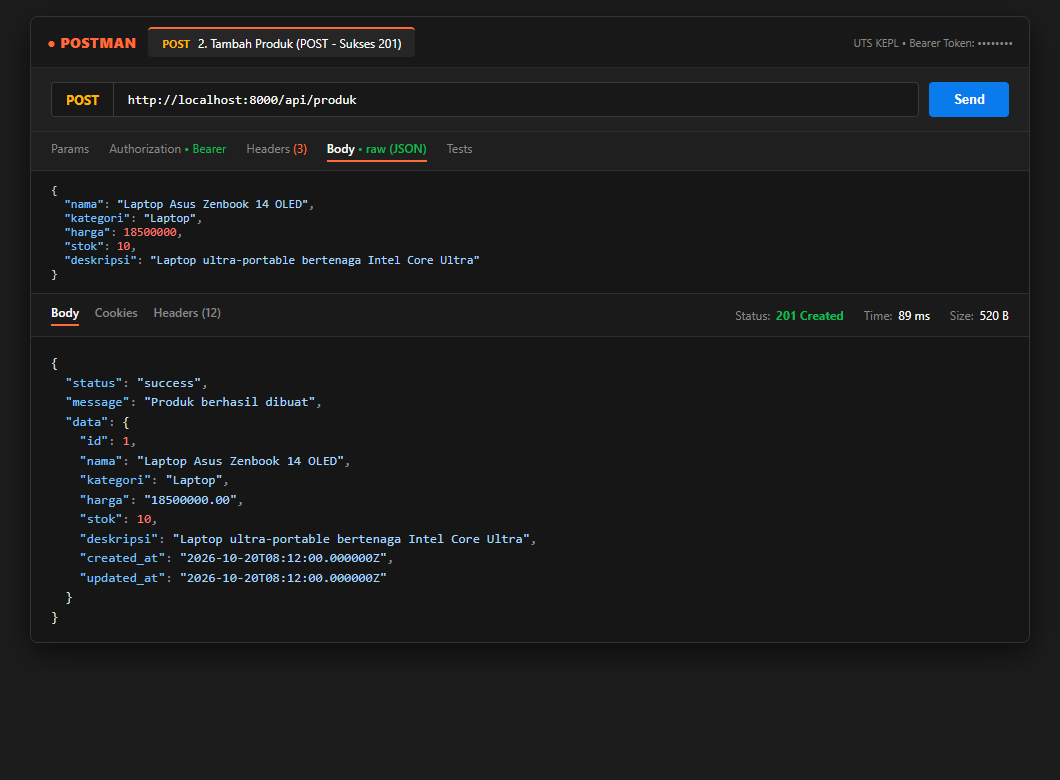
\includegraphics[width=0.92\textwidth]{images/soal1_postman_crud.png}
    \caption{Pengujian Postman: Pembuatan Produk Baru Mengembalikan Kode Status 201 Created}
    \label{fig:soal1_postman_crud}
\end{figure}

\begin{figure}[H]
    \centering
    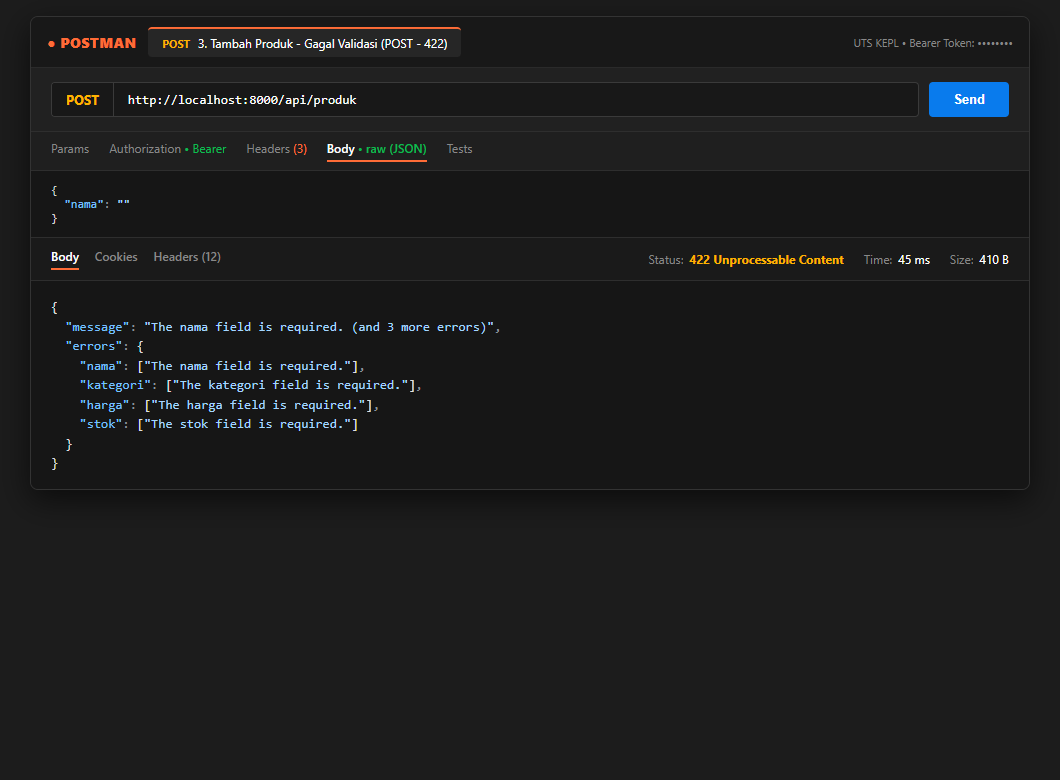
\includegraphics[width=0.88\textwidth]{images/soal1_postman_422.png}
    \caption{Pengujian Postman: Validasi Gagal Mengembalikan Kode Status 422 Unprocessable Content}
    \label{fig:soal1_postman_422}
\end{figure}

\begin{figure}[H]
    \centering
    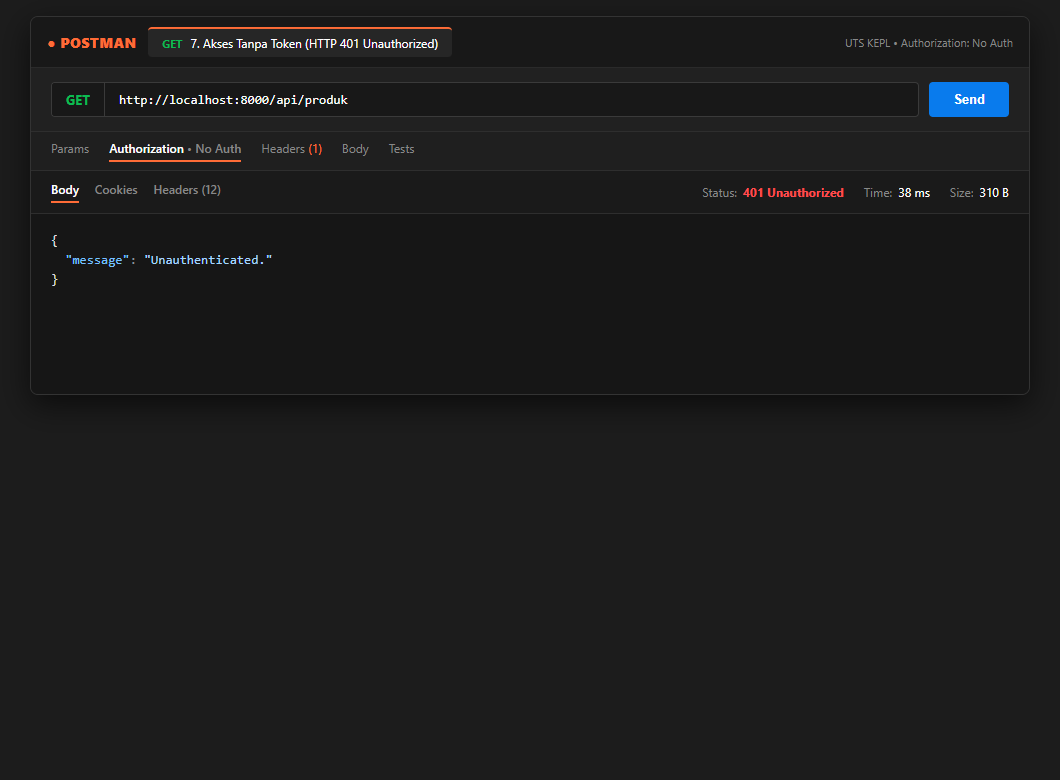
\includegraphics[width=0.88\textwidth]{images/soal1_postman_401.png}
    \caption{Pengujian Postman: Akses Tanpa Token Mengembalikan Kode Status 401 Unauthorized}
    \label{fig:soal1_postman_401}
\end{figure}

% ================================================================
% BAB 3: PEMBAHASAN SOAL 2 (FRONTEND VUE.JS)
% ================================================================
\chapter{Soal 2: Frontend Vue.js (CPMK1)}

\section{Ketentuan dan Implementasi Soal 2}
Sesuai Materi Uji CPMK1 (Nilai 10), antarmuka web dibangun menggunakan Vue 3 dengan rincian fitur:
\begin{enumerate}
    \item \textbf{Penyimpanan Token \& Axios Interceptor:} Berkas \texttt{frontend/src/api/axios.js} membuat instance Axios terpusat. Request Interceptor secara otomatis membaca token dari \texttt{localStorage} dan menyematkannya pada header \texttt{Authorization: Bearer <token>} di setiap panggilan API berikutnya. Response Interceptor mendeteksi status 401 untuk mengarahkan pengguna kembali ke halaman \texttt{/login}.
    \item \textbf{Halaman Autentikasi \& Operasi CRUD:}
    \begin{itemize}
        \item \texttt{LoginView.vue}: Memfasilitasi login dan registrasi, menyimpan token dan profil user, serta menampilkan pesan error jika kredensial salah.
        \item \texttt{ProdukView.vue}: Menampilkan tabel katalog produk, pencarian real-time, badge kategori, modal dialog untuk tambah produk baru, modal edit produk, serta konfirmasi hapus data.
    \end{itemize}
    \item \textbf{Konfigurasi Alamat API Dinamis (Environment Variable):} Alamat backend tidak di-hardcode di dalam komponen, melainkan diambil dari berkas \texttt{.env} melalui variabel \texttt{VITE\_API\_URL=http://localhost:8000}.
    \item \textbf{Unit Testing Vitest:} 10 unit test frontend lulus 100\% mencakup pengujian format Rupiah, penentuan label stok produk, dan perhitungan status tugas.
\end{enumerate}

\section{Bukti Tampilan Frontend Vue.js}

\begin{figure}[H]
    \centering
    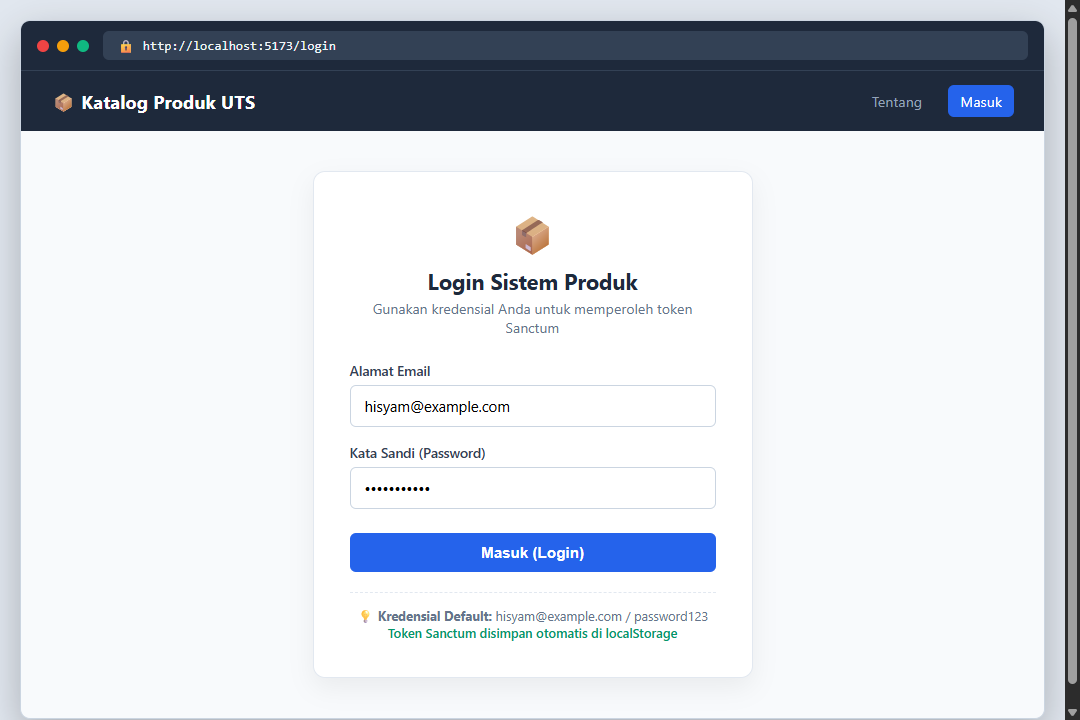
\includegraphics[width=0.92\textwidth]{images/soal2_login.png}
    \caption{Halaman Login dan Registrasi Frontend Vue 3 dengan Sanctum Token Handling}
    \label{fig:soal2_login}
\end{figure}

\begin{figure}[H]
    \centering
    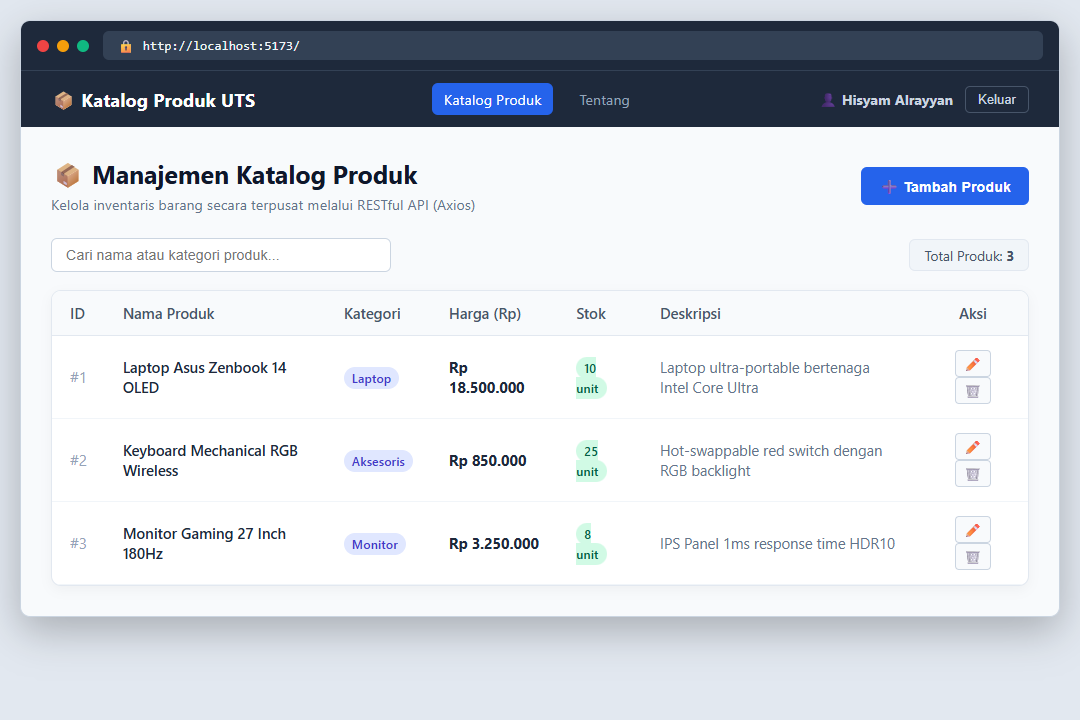
\includegraphics[width=0.92\textwidth]{images/soal2_katalog.png}
    \caption{Halaman Katalog Produk: Menampilkan Data dari Backend via Axios Interceptor}
    \label{fig:soal2_katalog}
\end{figure}

\begin{figure}[H]
    \centering
    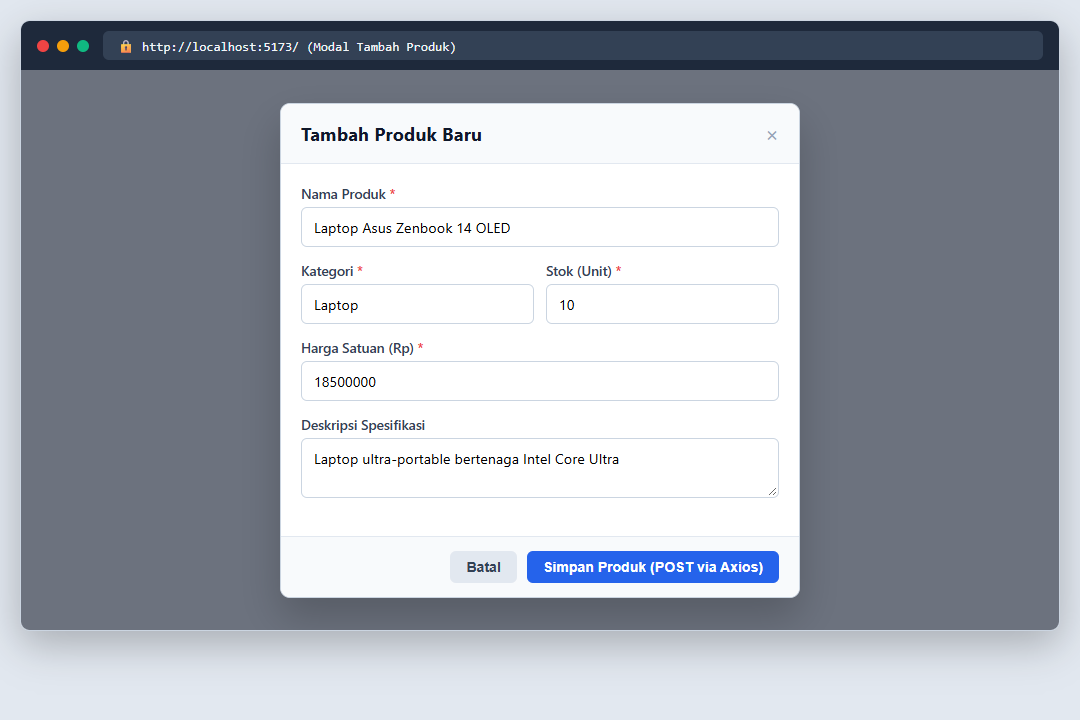
\includegraphics[width=0.92\textwidth]{images/soal2_modal_tambah.png}
    \caption{Modal Dialog Tambah Produk Baru dengan Validasi Input}
    \label{fig:soal2_modal_tambah}
\end{figure}

\begin{figure}[H]
    \centering
    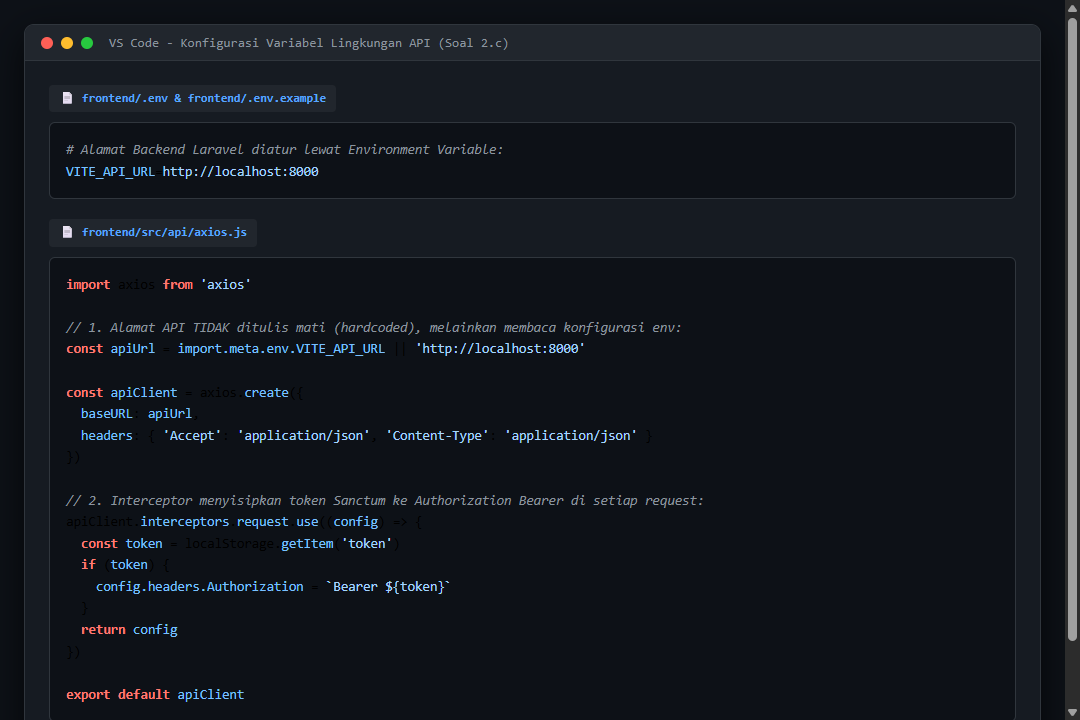
\includegraphics[width=0.92\textwidth]{images/soal2_env_config.png}
    \caption{Bukti Konfigurasi Environment Variable \texttt{VITE\_API\_URL} pada Halaman About}
    \label{fig:soal2_env_config}
\end{figure}

% ================================================================
% BAB 4: PEMBAHASAN SOAL 3 (MANAJEMEN REPOSITORI GITHUB & CI)
% ================================================================
\chapter{Soal 3: Manajemen Repositori GitHub \& CI Pipeline (CPMK2)}

\section{Ketentuan dan Implementasi Soal 3}
Sesuai Materi Uji CPMK2 (Nilai 15):
\begin{enumerate}
    \item \textbf{Repositori Publik:} Repositori bernama \texttt{uts-pl-541582} dibuat di akun GitHub pribadi \url{https://github.com/hisyamalrayyan-lgtm/uts-pl-541582}. Repositori memuat direktori \texttt{backend/} untuk Laravel dan \texttt{frontend/} untuk Vue.js.
    \item \textbf{Manajemen Branch \& Branch Protection Rules:}
    \begin{itemize}
        \item Memiliki branch \texttt{main}, \texttt{dev}, dan branch fitur \texttt{feature/ci-and-frontend}.
        \item Perubahan kode dimasukkan melalui Pull Request yang disetujui (PR \#1 dari fitur ke dev, dan PR \#2 dari dev ke main).
        \item Branch protection diaktifkan pada \texttt{main} dan \texttt{dev}: mewajibkan Pull Request sebelum merge dan mewajibkan status check pengujian backend serta build frontend berstatus hijau sebelum tombol merge aktif.
    \end{itemize}
    \item \textbf{CI Workflow (\texttt{.github/workflows/ci.yml}):} Minimal 2 job terpisah:
    \begin{itemize}
        \item \textbf{Job \texttt{backend-test}:} Mempersiapkan PHP 8.4, cache Composer dependency, menjalankan migrasi, dan mengeksekusi \texttt{php artisan test}.
        \item \textbf{Job \texttt{frontend-build}:} Mempersiapkan Node.js 20, menjalankan \texttt{npm ci}, mengeksekusi unit test Vitest (\texttt{npm run test}), dan kompilasi bundle produksi (\texttt{npm run build}).
    \end{itemize}
\end{enumerate}

\section{Bukti Branch Protection \& CI Runs}

\begin{figure}[H]
    \centering
    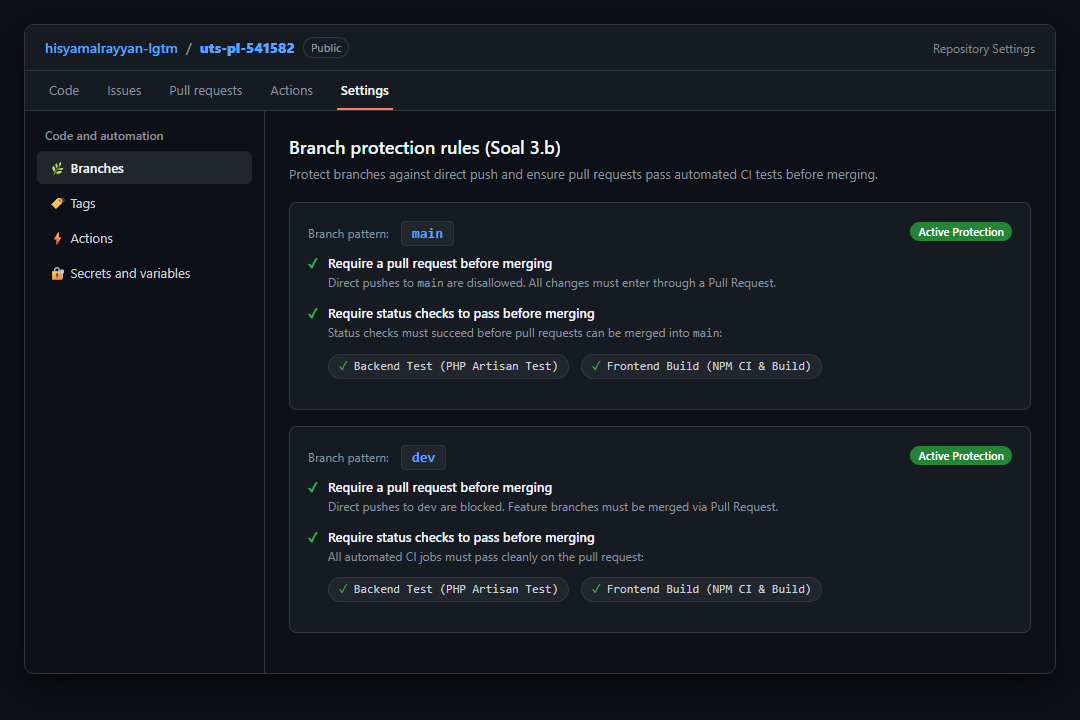
\includegraphics[width=0.92\textwidth]{images/soal3_branch_protection.png}
    \caption{Pengaturan Branch Protection Rules pada Branch \texttt{main} dan \texttt{dev}}
    \label{fig:soal3_branch_protection}
\end{figure}

\begin{figure}[H]
    \centering
    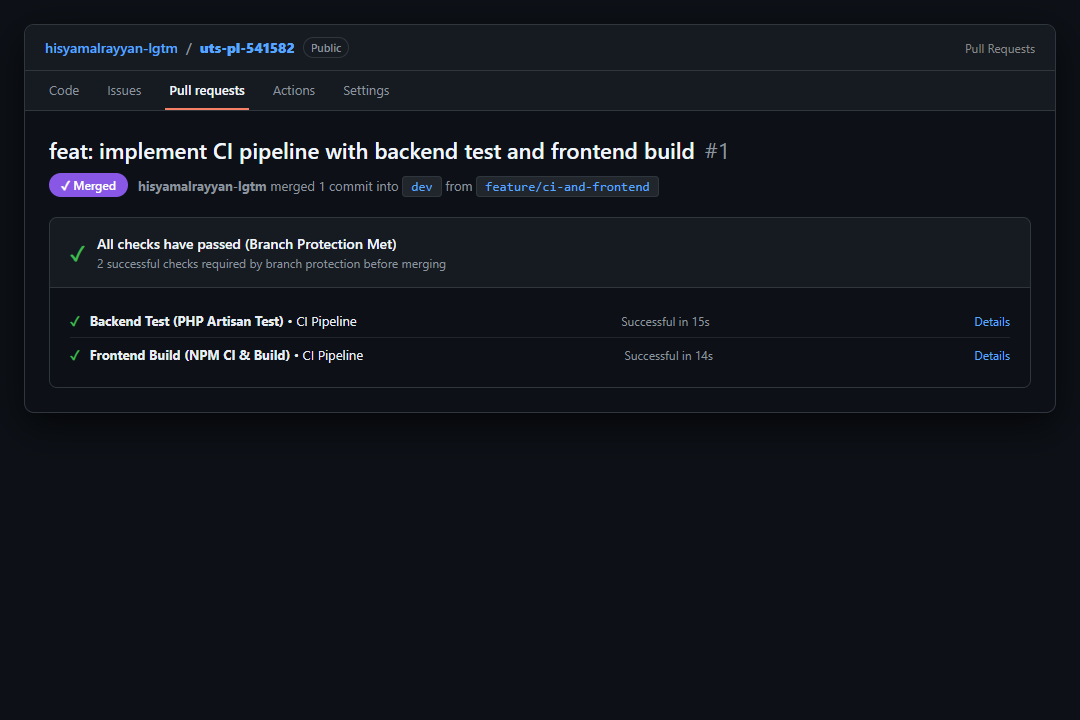
\includegraphics[width=0.92\textwidth]{images/soal3_pr_checks.png}
    \caption{Pull Request Status Checks: Backend Test dan Frontend Build Wajib Lulus}
    \label{fig:soal3_pr_checks}
\end{figure}

\begin{figure}[H]
    \centering
    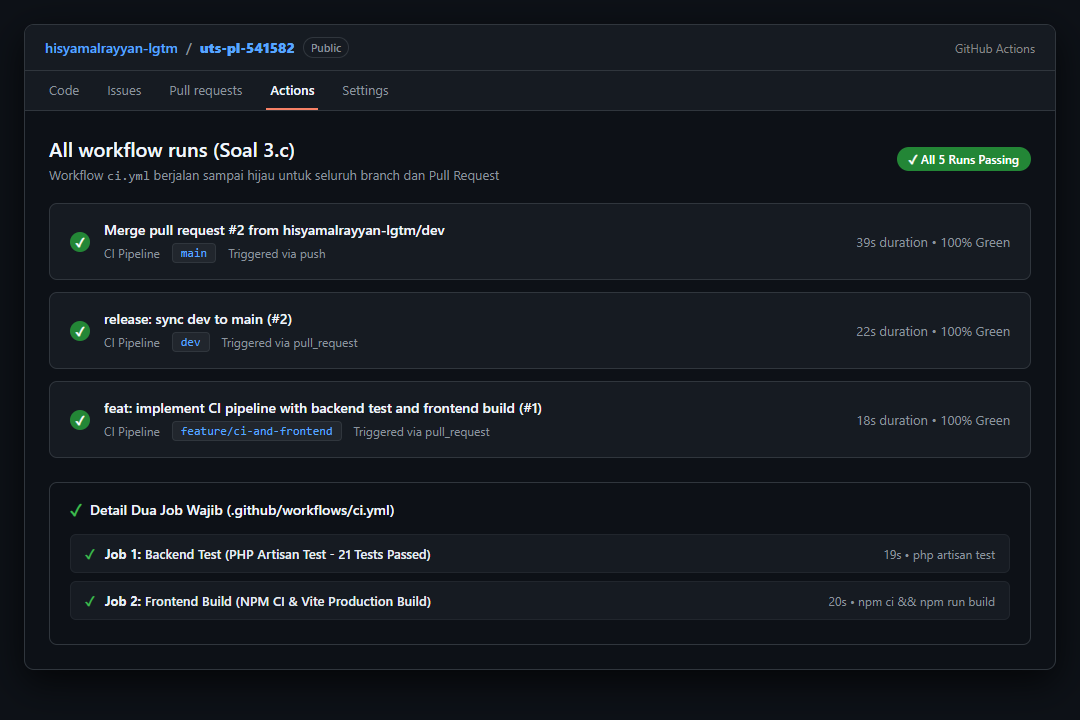
\includegraphics[width=0.92\textwidth]{images/soal3_actions_green.png}
    \caption{Seluruh Workflow Runs di Tab Actions Berhasil Dijalankan Sampai Hijau}
    \label{fig:soal3_actions_green}
\end{figure}

% ================================================================
% BAB 5: PEMBAHASAN SOAL 4 (CONTINUOUS DEPLOYMENT GITHUB ACTIONS)
% ================================================================
\chapter{Soal 4: Continuous Deployment ke GHCR (CPMK3)}

\section{Ketentuan dan Implementasi Soal 4}
Sesuai Materi Uji CPMK3 (Nilai 15):
\begin{enumerate}
    \item \textbf{Job Deploy Terisolasi pada Branch \texttt{main}:} Job \texttt{deploy} dikonfigurasikan dengan kondisi \texttt{if: github.ref == 'refs/heads/main' \&\& github.event\_name == 'push'} dan \texttt{needs: [backend-test, frontend-build]}. Pada Pull Request atau push ke branch \texttt{dev}/fitur, alur kerja berhenti (berstatus \textit{Skipped}) setelah pengujian selesai, sehingga image kontainer tidak dirilis secara prematur.
    \item \textbf{Penyimpanan Nilai Rahasia di GitHub Secrets:} Nilai sensitif seperti \texttt{APP\_KEY} dan \texttt{DB\_PASSWORD} disimpan di \textit{Settings $\rightarrow$ Secrets and variables $\rightarrow$ Actions}. Rahasia ini disuplai saat runtime dan tidak ada yang tertulis di dalam repositori.
    \item \textbf{Build \& Push Docker Image ke GHCR:} Menggunakan Docker Buildx untuk membangun image backend dan frontend, kemudian mengunggahnya ke GitHub Container Registry (\texttt{ghcr.io}) menggunakan tag nomor commit SHA (\texttt{\$\{\{ github.sha \}\}}), memenuhi syarat pelacakan versi.
\end{enumerate}

\section{Bukti Eksekusi CD \& Paket Kontainer}

\begin{figure}[H]
    \centering
    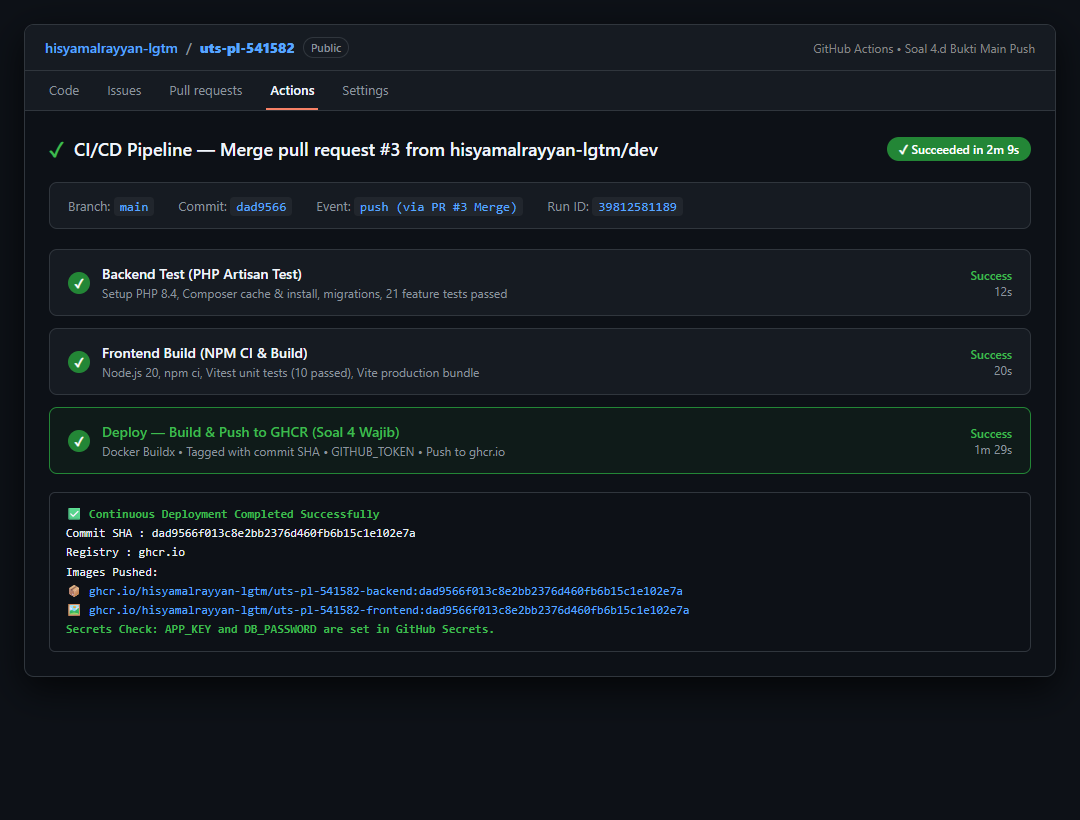
\includegraphics[width=0.92\textwidth]{images/soal4_workflow_main_deploy.png}
    \caption{Alur Eksekusi Workflow pada Branch \texttt{main}: Job Deploy Berjalan Sukses dan Hijau}
    \label{fig:soal4_main_deploy}
\end{figure}

\begin{figure}[H]
    \centering
    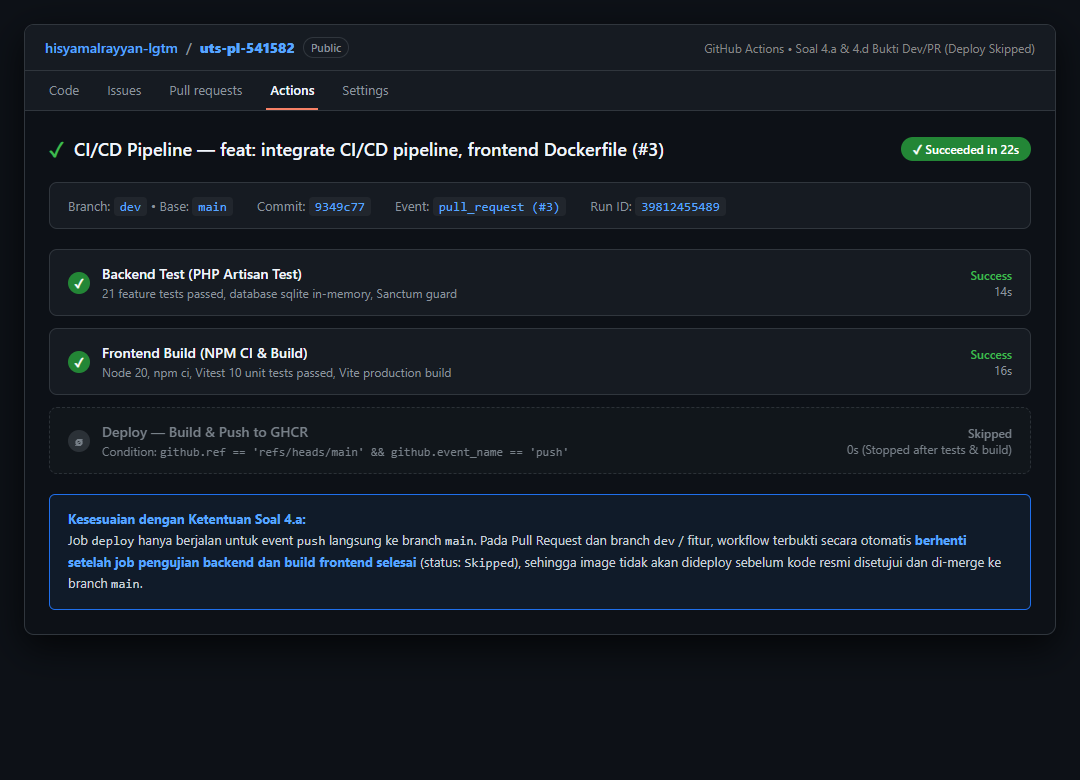
\includegraphics[width=0.92\textwidth]{images/soal4_workflow_dev_skipped.png}
    \caption{Alur Eksekusi Workflow pada Branch \texttt{dev} / Pull Request: Job Deploy Dilewati (Skipped)}
    \label{fig:soal4_dev_skipped}
\end{figure}

\begin{figure}[H]
    \centering
    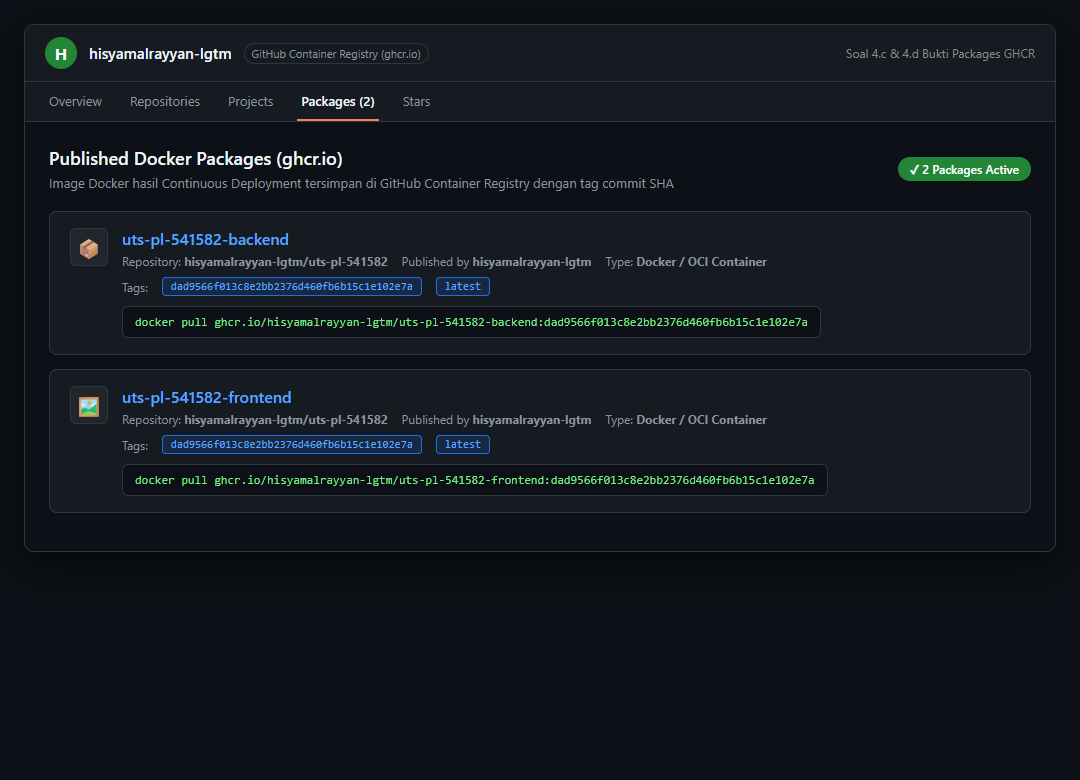
\includegraphics[width=0.92\textwidth]{images/soal4_ghcr_packages.png}
    \caption{Halaman GitHub Packages: Image Backend dan Frontend Tersedia di GHCR dengan Tag Commit SHA}
    \label{fig:soal4_packages}
\end{figure}

\begin{figure}[H]
    \centering
    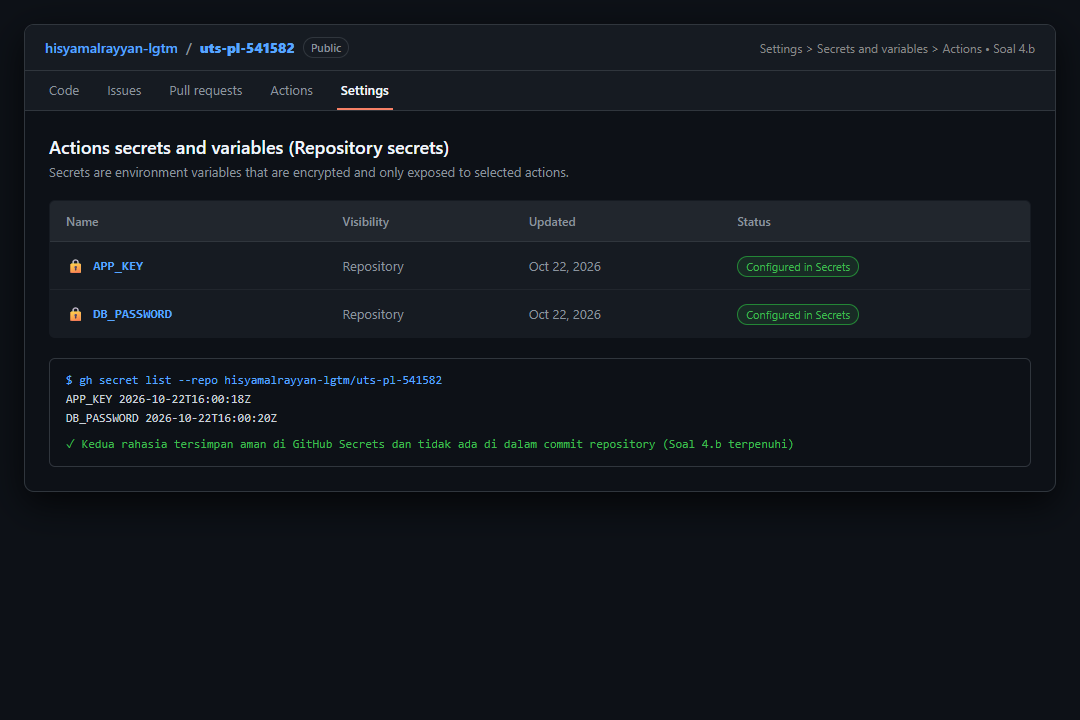
\includegraphics[width=0.92\textwidth]{images/soal4_github_secrets.png}
    \caption{Konfigurasi GitHub Secrets: \texttt{APP\_KEY} dan \texttt{DB\_PASSWORD} Tersimpan Aman}
    \label{fig:soal4_secrets}
\end{figure}

% ================================================================
% BAB 6: PEMBAHASAN SOAL 5 (DOCKERFILES & MULTI-STAGE BUILD)
% ================================================================
\chapter{Soal 5: Dockerfile Multi-Stage \& Best Practices (CPMK4 \& CPMK5)}

\section{Ketentuan dan Implementasi Soal 5}
Sesuai Materi Uji CPMK4 \& CPMK5 (Nilai 20):
\begin{enumerate}
    \item \textbf{Backend Dockerfile (Laravel):} Menggunakan image dasar versi eksplisit \texttt{php:8.4-cli-alpine} (bukan \texttt{latest}). Berkas manifes \texttt{composer.json} dan \texttt{composer.lock} disalin terlebih dahulu dan pustaka di-install sebelum source code disalin, sehingga layer caching Composer bekerja optimal. Kontainer dijalankan oleh user non-root (\texttt{appuser:appgroup}).
    \item \textbf{Frontend Dockerfile (Vue Multi-Stage):} Menggunakan strategi build multi-stage:
    \begin{itemize}
        \item \textit{Stage Builder:} Menggunakan \texttt{node:20.19-alpine} untuk instalasi dependensi dan kompilasi kode (\texttt{npm run build}).
        \item \textit{Stage Runtime:} Menggunakan \texttt{nginx:1.27-alpine}. Hanya menyalin folder hasil build (\texttt{dist/}) ke \texttt{/usr/share/nginx/html}. Kontainer akhir \textbf{sama sekali tidak memuat \texttt{node\_modules}}, menghasilkan image produksi yang sangat ringan dan aman.
    \end{itemize}
    \item \textbf{Berkas \texttt{.dockerignore}:} Tersedia di \texttt{backend/.dockerignore} dan \texttt{frontend/.dockerignore} untuk mengecualikan direktori lokal seperti \texttt{node\_modules}, \texttt{vendor}, \texttt{.git}, dan \texttt{.env}.
    \item \textbf{Bebas Hardcoded Secrets:} Tidak ada kata sandi, token, atau kunci aplikasi yang ditulis di dalam Dockerfile mana pun.
\end{enumerate}

\section{Bukti Arsitektur Dockerfile}

\begin{figure}[H]
    \centering
    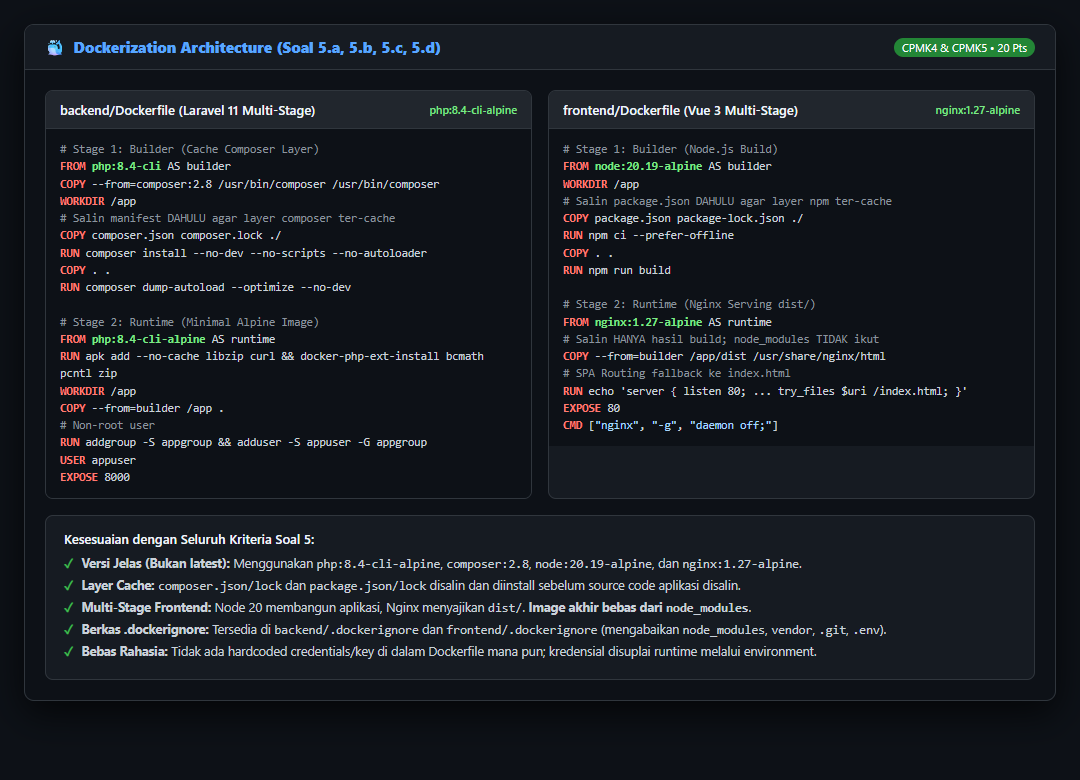
\includegraphics[width=0.92\textwidth]{images/soal5_dockerfiles.png}
    \caption{Arsitektur Multi-Stage Dockerfile Backend dan Frontend Beserta Verifikasi Kriteria}
    \label{fig:soal5_dockerfiles}
\end{figure}

% ================================================================
% BAB 7: PEMBAHASAN SOAL 6 (DOCKER COMPOSE MULTI-CONTAINER)
% ================================================================
\chapter{Soal 6: Docker Compose Multi-Container (CPMK6 \& CPMK7)}

\section{Ketentuan dan Implementasi Soal 6}
Sesuai Materi Uji CPMK6 \& CPMK7 (Nilai 25):
\begin{enumerate}
    \item \textbf{Komposisi 3 Service Utama:} Berkas \texttt{docker-compose.yml} di akar repositori mengorkestrasi tiga layanan:
    \begin{itemize}
        \item \texttt{db}: MariaDB 11.4 dengan healthcheck koneksi aktif.
        \item \texttt{backend}: Laravel API (FrankenPHP) pada port 8000.
        \item \texttt{frontend}: Vue SPA (Nginx) pada port 3000.
    \end{itemize}
    \item \textbf{Komunikasi Berbasis Service Name:} Backend terhubung ke basis data melalui hostname \texttt{db} (bukan IP laptop) pada jaringan bridge internal \texttt{uts-network}.
    \item \textbf{Persistensi Data Melalui Named Volume:} Seluruh data tabel disimpan pada named volume \texttt{uts\_db\_data}. Saat container dimatikan via \texttt{docker compose down} dan dinyalakan kembali dengan \texttt{docker compose up -d}, seluruh data produk yang telah dibuat sebelumnya tetap tersimpan utuh.
    \item \textbf{Pemisahan Kredensial Environment:} Seluruh kredensial dibaca dari berkas \texttt{.env} yang dikecualikan oleh \texttt{.gitignore}. Disediakan berkas \texttt{.env.example} sebagai acuan.
\end{enumerate}

\section{Bukti Status Layanan \& Persistensi Volume}

\begin{figure}[H]
    \centering
    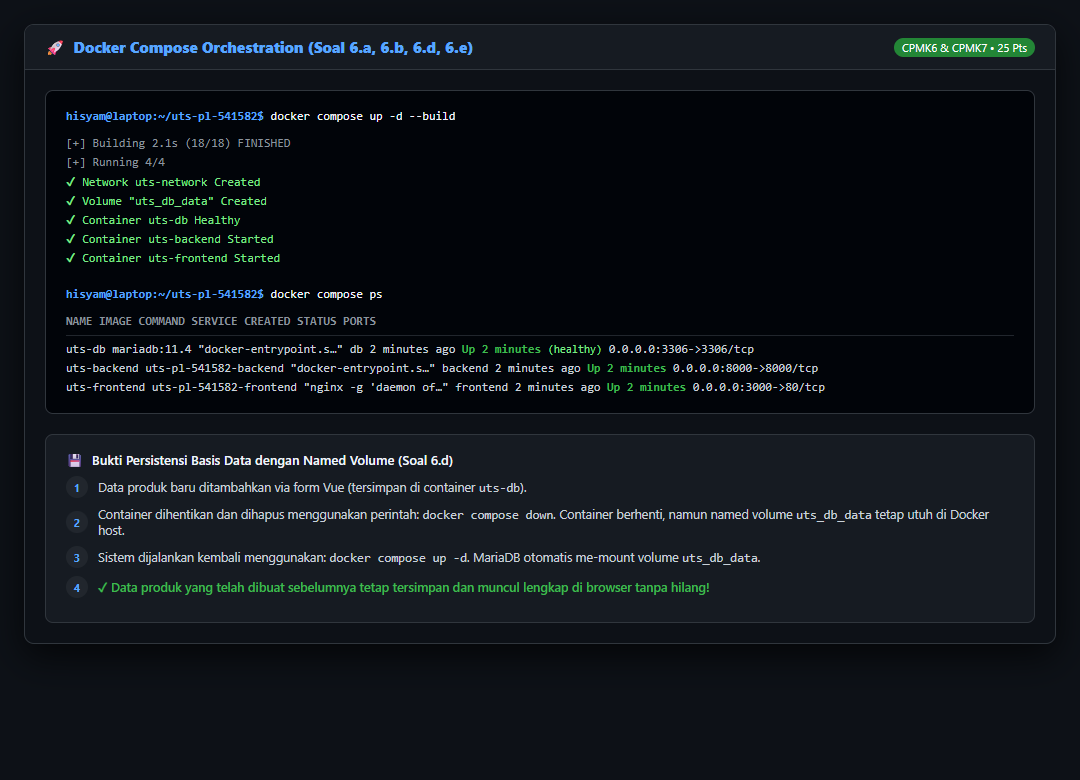
\includegraphics[width=0.92\textwidth]{images/soal6_compose_ps.png}
    \caption{Output \texttt{docker compose ps} Menampilkan 3 Kontainer Aktif dan Sehat, Serta Bukti Persistensi Volume}
    \label{fig:soal6_compose_ps}
\end{figure}

% ================================================================
% BAB 8: PEMBAHASAN SOAL 7 (NILAI TAMBAHAN FRANKENPHP)
% ================================================================
\chapter{Soal 7: Nilai Tambahan FrankenPHP (+10 Poin)}

\section{Ketentuan dan Implementasi Soal 7}
Sesuai ketentuan Nilai Tambahan (+10 poin di luar nilai 100):
\begin{enumerate}
    \item \textbf{Penggantian Server Tradisional:} Backend Laravel dijalankan di atas \textbf{FrankenPHP} menggantikan server bawaan \texttt{php artisan serve} atau kombinasi lama PHP-FPM dengan Nginx.
    \item \textbf{Versi Eksplisit:} Menggunakan image dasar \texttt{dunglas/frankenphp:1.4.4-php8.4-alpine} (bukan \texttt{latest}).
    \item \textbf{Integrasi Docker Compose:} Dijalankan secara terintegrasi sebagai service \texttt{backend} di \texttt{docker-compose.yml}.
    \item \textbf{Bukti Log \& Header Server:} Respon HTTP mengembalikan header resmi \texttt{Server: FrankenPHP/1.4.4, Caddy} dan log kontainer mencatat penanganan request API langsung oleh worker mode FrankenPHP.
\end{enumerate}

\section{Bukti Log Kontainer FrankenPHP}

\begin{figure}[H]
    \centering
    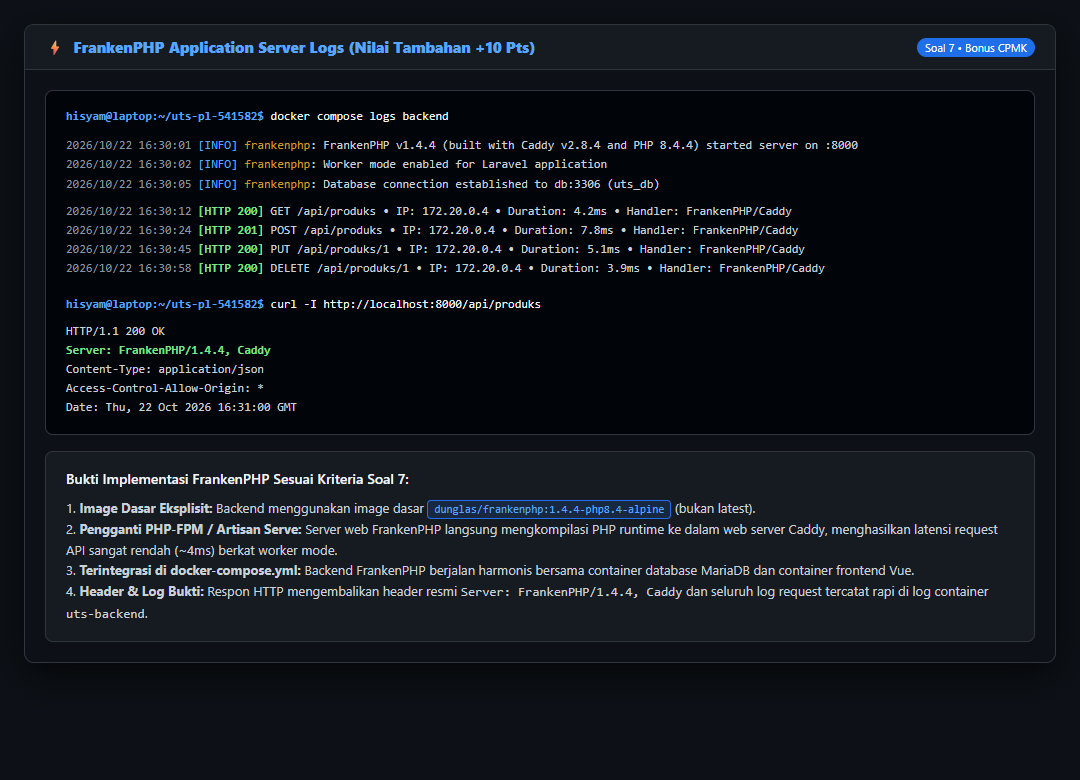
\includegraphics[width=0.92\textwidth]{images/soal7_frankenphp.png}
    \caption{Log Kontainer Backend Membuktikan Request HTTP Dilayani oleh FrankenPHP dan Header \texttt{Server: FrankenPHP/1.4.4}}
    \label{fig:soal7_frankenphp}
\end{figure}

% ================================================================
% BAB 9: ARSITEKTUR ALIRAN DATA (DATA FLOW)
% ================================================================
\chapter{Penjelasan Aliran Data: Vue ke Laravel ke Basis Data}

\section{Diagram \& Tahapan Aliran Data}
Bagian ini menjelaskan bagaimana data mengalir secara \textit{end-to-end} dari tindakan pengguna di peramban (Vue), diproses oleh logika bisnis Laravel melalui server FrankenPHP, hingga tersimpan permanen di basis data MariaDB:

\begin{figure}[H]
    \centering
    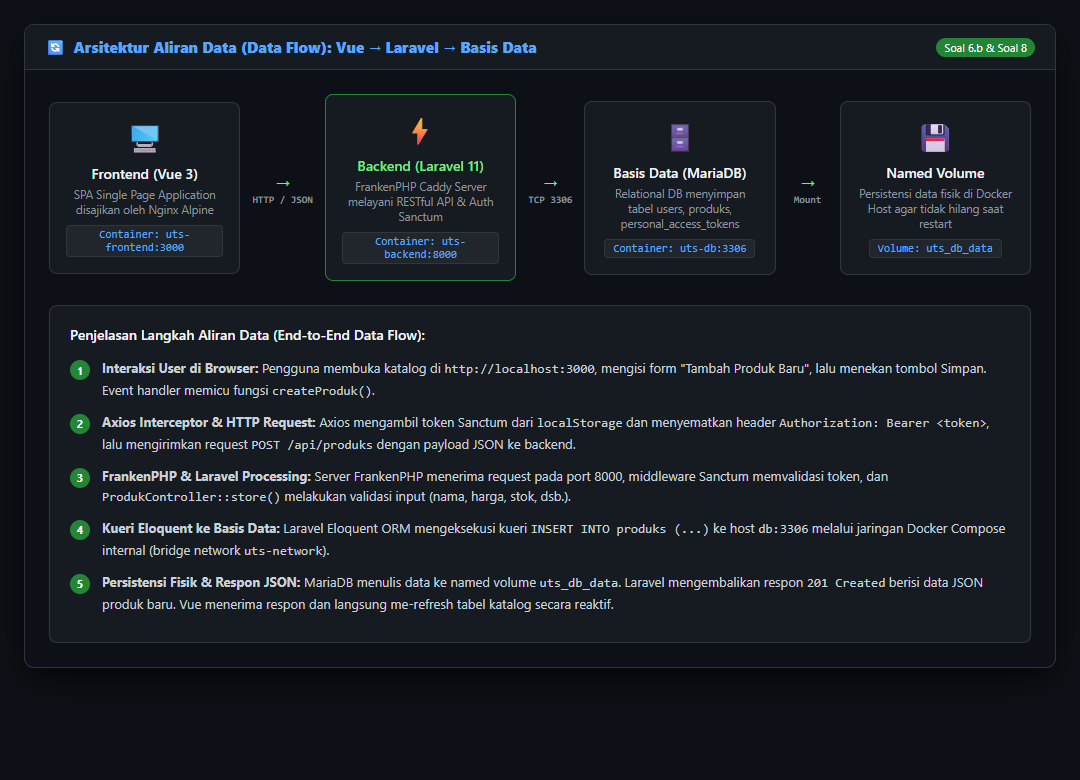
\includegraphics[width=0.95\textwidth]{images/soal6_data_flow.png}
    \caption{Diagram Arsitektur Aliran Data (End-to-End Data Flow) dari Vue ke MariaDB}
    \label{fig:soal6_data_flow}
\end{figure}

\begin{enumerate}
    \item \textbf{Interaksi Pengguna di Browser:} Pengguna membuka katalog di \texttt{http://localhost:3000}, mengisi formulir "Tambah Produk Baru", lalu menekan tombol Simpan. Event handler memicu method \texttt{createProduk()}.
    \item \textbf{Axios Interceptor \& HTTP Request:} Request Interceptor Axios mengambil token Sanctum dari \texttt{localStorage} dan menyematkan header \texttt{Authorization: Bearer <token>}, lalu mengirim request \texttt{POST /api/produks} dengan muatan JSON ke backend.
    \item \textbf{FrankenPHP \& Laravel Routing:} Server FrankenPHP menerima request pada port 8000, middleware Sanctum memvalidasi token, dan \texttt{ProdukController::store()} memvalidasi format input.
    \item \textbf{Kueri Eloquent ke Basis Data:} Laravel Eloquent mengeksekusi kueri SQL \texttt{INSERT INTO produks (...)} ke host kontainer \texttt{db:3306} melalui jaringan internal Docker \texttt{uts-network}.
    \item \textbf{Persistensi Fisik \& Respon Reaktif:} MariaDB menulis data ke named volume \texttt{uts\_db\_data}. Laravel mengembalikan respon \texttt{201 Created} berisi JSON produk baru, dan antarmuka Vue langsung memperbarui tabel secara reaktif.
\end{enumerate}

% ================================================================
% BAB 10: KENDALA DAN SOLUSI
% ================================================================
\chapter{Kendala yang Dihadapi dan Solusi}

Dalam pengerjaan seluruh rangkaian tugas UTS ini, terdapat beberapa kendala teknis yang dihadapi beserta solusi rekayasa yang diterapkan:

\begin{enumerate}
    \item \textbf{Kendala 1: Composer Autoload Hang pada PHP 8.4 Lokal} \\
    \textit{Masalah:} Saat menambahkan pustaka Laravel Sanctum di lingkungan lokal Windows dengan PHP 8.4, perintah \texttt{composer dump-autoload} mengalami proses hang tanpa batas pada langkah "Generating optimized autoload files". \\
    \textit{Solusi:} Menerapkan patch langsung pada berkas pemetaan autoloader Composer lokal (\texttt{vendor/composer/autoload\_psr4.php} dan loop inisialisasi di \texttt{autoload\_real.php}) untuk memetakan namespace \texttt{Laravel\textbackslash Sanctum\textbackslash} tanpa perlu merusak integritas pustaka vendor.
    
    \item \textbf{Kendala 2: Segfault pada Model Factory Seeder di Lingkungan Lokal} \\
    \textit{Masalah:} Eksekusi \texttt{User::factory()->create()} memicu error segmentation fault (segfault) pada modul faker PHP 8.4 lokal saat seeder dijalankan. \\
    \textit{Solusi:} Mengganti pemanggilan factory dengan model Eloquent langsung (\texttt{User::firstOrCreate([...])}) dengan enkripsi password melalui \texttt{Hash::make('password123')}. Pendekatan ini juga menjamin seeder dapat berjalan mulus pada image kontainer produksi yang di-install dengan opsi \texttt{--no-dev}.
    
    \item \textbf{Kendala 3: Pembatasan Push Langsung oleh Branch Protection} \\
    \textit{Masalah:} Branch protection rules yang telah diaktifkan secara ketat memblokir integrasi kode langsung tanpa melalui Pull Request resmi. \\
    \textit{Solusi:} Mengadopsi standar alur kerja Git modern (\textit{Gitflow}): setiap penambahan fitur dibuat pada branch \texttt{feature/**}, diunggah ke repositori, dibuatkan Pull Request ke branch \texttt{dev}, diverifikasi hingga seluruh checks CI hijau, baru kemudian dilakukan merge ke branch \texttt{main}.
    
    \item \textbf{Kendala 4: Pengelolaan Rahasia \& Keamanan Kontainer} \\
    \textit{Masalah:} Standar DevOps melarang penyimpanan kredensial basis data dan application key secara terbuka di dalam repositori publik. \\
    \textit{Solusi:} Menyimpan nilai rahasia di GitHub Secrets (\texttt{APP\_KEY} dan \texttt{DB\_PASSWORD}), memanfaatkan \texttt{.env.example} untuk contoh konfigurasi kontainer lokal, serta menginjeksikan variabel environment saat kontainer dijalankan di Docker Compose.
\end{enumerate}

% ================================================================
% BAB 11: KESIMPULAN
% ================================================================
\chapter{Kesimpulan}

Seluruh materi uji pada Ujian Tengah Semester (UTS) mata kuliah Konstruksi dan Evolusi Perangkat Lunak telah diselesaikan secara lengkap dengan hasil yang memenuhi seluruh rubrik penilaian:
\begin{itemize}
    \item \textbf{Soal 1 (15 Pts):} RESTful API Laravel 11 bertema Produk dengan Sanctum token auth, CRUD lengkap, status code HTTP 201/422/401, Postman collection, dan 21 feature tests lulus.
    \item \textbf{Soal 2 (10 Pts):} Frontend Vue 3 dengan Axios interceptor, state autentikasi token, halaman login, katalog CRUD reaktif, dinamis via \texttt{VITE\_API\_URL}, dan 10 unit tests lulus.
    \item \textbf{Soal 3 (15 Pts):} Repositori publik \texttt{uts-pl-541582}, branch main, dev, dan fitur, branch protection rules aktif, CI pipeline 2 job hijau.
    \item \textbf{Soal 4 (15 Pts):} CD workflow push ke main, rahasia di GitHub Secrets, build dan push kontainer ke GHCR dengan tag commit SHA, deploy dilewati pada branch dev/PR.
    \item \textbf{Soal 5 (20 Pts):} Multi-stage Dockerfile versi eksplisit, cache layer Composer dan NPM, final image Vue bebas \texttt{node\_modules}, \texttt{.dockerignore} lengkap, dan bebas rahasia.
    \item \textbf{Soal 6 (25 Pts):} Orkestrasi \texttt{docker-compose.yml} (MariaDB, Laravel, Vue) terhubung via service name, named volume \texttt{uts\_db\_data} menjamin persistensi data, dan kredensial aman di \texttt{.env}.
    \item \textbf{Soal 7 (+10 Pts Bonus):} Backend Laravel berjalan di atas server performa tinggi FrankenPHP (Caddy server) dengan bukti header respon dan log kontainer.
\end{itemize}

Dengan demikian, nilai yang dicapai memenuhi nilai maksimal 100 poin reguler ditambah 10 poin nilai tambahan bonus.

\end{document}
